\chapter{Automatisation du processus d'investigation}
\label{Automatisation du processus d'investigation}
\thispagestyle{fancy}


\section{Architecture High Level du système proposé}
\label{Automatisation du processus d'investigation: Achitecture High Level du système proposé}
On présente l'architecture haut niveau de notre système permettant l'automatisation de la phase d'investigation des erreurs issues du Filtering Test. On réalise également une analyse de chacune des sous partie du système (i.e. exemples pour l'entrainement, exemple à analyser, modèle d'apprentissage, décision).

\subsubsection{Schéma synoptique High Level}
\label{Automatisation du processus d'investigation: Achitecture High Level du système proposé: Schéma synoptique High Level}
En s'appuyant sur les définitions et l'architecture High Level du Machine Learning (partie \ref{Le Machine Learning: Généralités sur le Machine Learning: Définition et principe général}), on propose un schéma synoptique haut niveau de la solution proposée (figure, en réponse à la problématique. 

\begin{figure}[h]
	\centering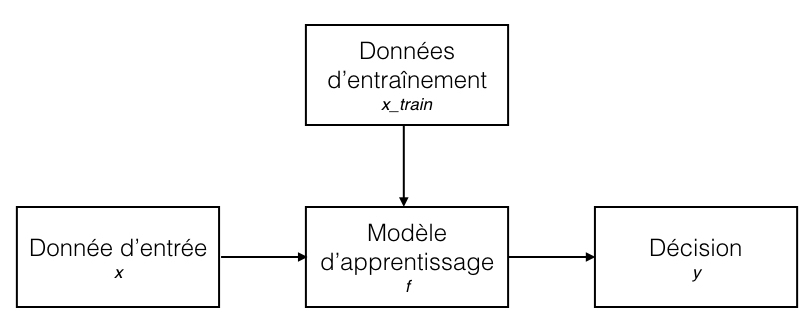
\includegraphics[height=5cm]{images/ML_high_level.jpeg}
	\caption{Schéma synoptique haut niveau de la solution proposée}
	\label{fig:Schéma synoptique haut niveau de la solution proposée}
\end{figure}

\subsubsection{Les exemples d'apprentissage et exemple à analyser}
\label{Automatisation du processus d'investigation: Achitecture High Level du système proposé: Les exemples d'apprentissage}

\subsubsection{Le modèle d'apprentissage}
\label{Automatisation du processus d'investigation: Achitecture High Level du système proposé: Le modèle d'apprentissage}

\subsubsection{La décision}
\label{Automatisation du processus d'investigation: Achitecture High Level du système proposé: La décision}

\section{Solutions techniques testées}
\label{Automatisation du processus d'investigation: Solutions techniques testées}




\section{Solution technique proposée}
\label{Automatisation du processus d'investigation: Solution technique proposée}

